% Uses the course-supplied IEEEtran journal template and its eleven sections.
% Technical draft: Kaggle scores supplied on 2026-11-16; team name, personal reflections, category-hour breakdown, attestation and Top-5 interpretation remain pending.
\documentclass[journal]{IEEEtran}
\usepackage{amsmath,amsfonts}
\usepackage{algorithmic}
\usepackage{algorithm}
\usepackage{array}
\usepackage[caption=false,font=normalsize,labelfont=sf,textfont=sf]{subfig}
\usepackage{textcomp,stfloats,url,verbatim,graphicx,cite,tabularx,booktabs}
\usepackage[hidelinks]{hyperref}
\usepackage{iftex}
\ifPDFTeX
  \usepackage[T1]{fontenc}
  \usepackage{mathptmx}
\else
  \usepackage{fontspec}
  \setmainfont{texgyretermes-regular.otf}[BoldFont=texgyretermes-bold.otf,ItalicFont=texgyretermes-italic.otf,BoldItalicFont=texgyretermes-bolditalic.otf]
  \setsansfont{texgyreheros-regular.otf}[BoldFont=texgyreheros-bold.otf,ItalicFont=texgyreheros-italic.otf,BoldItalicFont=texgyreheros-bolditalic.otf]
  \setmonofont{lmmono10-regular.otf}
\fi
\graphicspath{{../results/}}
\newcommand{\pending}[1]{\textbf{[Pending: #1]}}
\hyphenation{op-tical net-works semi-conduc-tor IEEE-Xplore}
\begin{document}
\title{CS4486 AI Course -- Mini Project Final Report:\\Statoil/C-CORE Iceberg Classifier Challenge}
\author{\textbf{Team Name:} [To be supplied]\\[1em]
Group Leader: Huang Yifan + 72400438\\
Group Member A: Zheng Hongyu + 72400229\\
Group Member B: Hachiware + 72400463}
\markboth{CS4486 AI Course - Mini Project Final Report - Technical Draft}{Radar Iceberg Classification}
\maketitle
\begin{abstract}
This project studies binary iceberg classification from two radar image channels and incidence-angle metadata. A compact convolutional network establishes an image-only baseline, followed by six controlled configurations evaluated on frozen five-fold splits. The experiments examine image flips, dropout, angle fusion and a missing-angle indicator. The selected configuration achieves a pooled out-of-fold Log Loss of 0.22683 and accuracy of 90.84\%. Its observed-angle loss is 0.24584. A supplementary angle-group protocol yields losses of 0.23123 overall and 0.25042 for observed angles. Error analysis identifies 147 classification errors, including 25 highly confident errors. All 45 handed-off checkpoints pass numerical prediction replay. Averaging five selected fold models produces 8,424 test predictions. A completed Kaggle late submission receives public Log Loss of 0.21791 and private Log Loss of 0.20895. These platform scores are distinct from development-validation scores; no formal leaderboard rank or Top-5 achievement is claimed. Code repository: \url{https://github.com/YifanHuang-if/cs4486-iceberg}.
\end{abstract}
\begin{IEEEkeywords}
Radar imagery, iceberg classification, multimodal learning, cross-validation, error analysis.
\end{IEEEkeywords}

\section{Task Description \& Metric}
\subsection{Problem and motivation}
The selected intermediate-tier course task is the Statoil/C-CORE Iceberg Classifier Challenge. The competition asks whether a remotely sensed target is a ship or an iceberg. Its input combines two radar bands with a numerical incidence angle, making it suitable for studying whether metadata complements learned image features. The competition website and official evaluation definition are cited in \cite{kaggle}.

Each input image contains two $75\times75$ arrays. The arrays represent HH and HV radar backscatter in decibels, rather than ordinary RGB intensity values. The numerical angle describes viewing geometry. These inputs motivate a convolutional image encoder and a separate small metadata branch. The target $y_i$ equals one for an iceberg and zero for a ship. A model produces $p_i=P(y_i=1\mid x_i,a_i)$, where $x_i$ denotes both image channels and $a_i$ denotes the angle and, where enabled, its missingness flag.

\subsection{Evaluation and interpretation}
The official metric is binary Log Loss. Our implementation uses natural logarithms and clips probabilities to \mbox{$[10^{-7},\,1-10^{-7}]$} for numerical evaluation:
\begin{equation}
L=-\frac{1}{N}\sum_{i=1}^{N}\left[y_i\log p_i+(1-y_i)\log(1-p_i)\right].
\end{equation}
Lower values indicate better probabilistic predictions. An incorrect prediction with high confidence receives a large penalty. For example, assigning probability 0.01 to a true iceberg contributes approximately 4.605 to the unaveraged loss. This explains why error analysis must inspect predicted probabilities as well as thresholded labels.

Accuracy uses a fixed threshold of 0.5 and is supplementary. No threshold was tuned to improve the reported accuracy. The submission file contains probabilities, not thresholded predictions. Local validation, final test inference and Kaggle scoring are distinct stages. All three have now been completed, with public and private late-submission scores recorded separately. The instructor's operational interpretation of the Top-5 target for a late submission remains to be confirmed.

\section{Data Analysis \& Challenges}
\subsection{Dataset profile}
The retained EDA records describe 1,604 training examples: 851 ships and 753 icebergs. The test set contains 8,424 examples. Each channel has 5,625 finite values, and the sample submission IDs match the test IDs in order. The class proportions are 53.05\% ships and 46.95\% icebergs, indicating modest class imbalance. Table~\ref{tab:data} summarizes the main data properties.

\begin{table}[t]
\caption{Dataset profile from the shared EDA and final input checks}
\label{tab:data}\centering
\begin{tabular}{lrr}\toprule
Property & Training & Test\\\midrule
Samples & 1,604 & 8,424\\
Ships / icebergs & 851 / 753 & Unknown\\
Image shape & $2\times75\times75$ & $2\times75\times75$\\
Missing angles & 133 & 0\\
Observed angle minimum & 24.7546 & 23.0805\\
Observed angle maximum & 45.9375 & 50.6618\\\bottomrule
\end{tabular}
\end{table}

\subsection{Missingness and distribution differences}
All 133 training examples with missing angles are ships. Missingness therefore provides a strong association with the label. However, the test set has no missing angles. An overall validation improvement from a missingness indicator can consequently overstate the expected improvement on test examples. We retain these samples and explicitly evaluate the 1,471 observed-angle examples separately from the 133 missing-angle examples.

Observed training angles span 24.7546--45.9375 degrees, whereas test angles span approximately 23.0805--50.6618 degrees. Predictions beyond the observed training range require extrapolation. The retained EDA also records differences in per-image means: median band-1 means are -21.0498 for training and -22.9298 for test, while median band-2 means are -26.1531 and -24.9241. These are descriptive distribution differences; they do not identify the physical cause or establish target-domain accuracy.

The official data description notes that some test images are machine-generated and excluded from scoring \cite{data}. Their identities are not used to remove rows. Predictions are supplied for every test ID. Consequently, aggregate statistics over the entire test file should not be treated as direct estimates of the scored subset's distribution.

\begin{figure*}[t]
\centering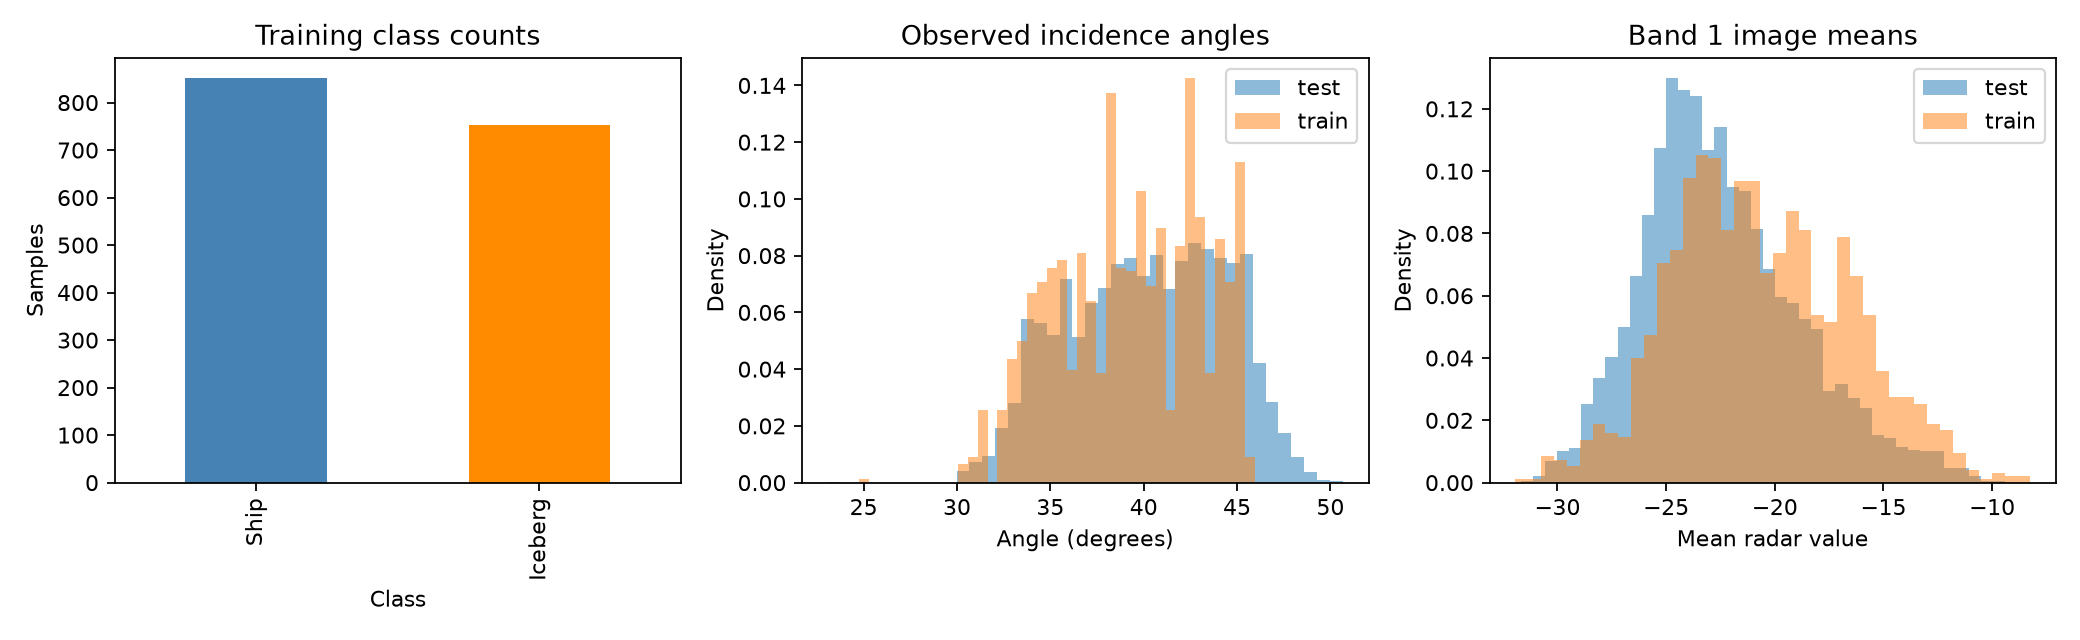
\includegraphics[width=.95\textwidth]{eda/distributions.png}
\caption{Shared EDA: class balance, angle distributions and image intensity summaries. These motivate subgroup evaluation and careful preprocessing.}
\label{fig:eda}
\end{figure*}

\subsection{Similarity review and preprocessing decisions}
The EDA found no repeated IDs, shared training/test IDs or exact two-channel duplicate images. A thumbnail-based screening procedure retained 182 similar-image candidate pairs. Subsequent full-resolution checks, after separately centering each channel, produced a maximum minimum-channel correlation of 0.849112, below the screening threshold of 0.98. No candidate met that additional grouping criterion.

This review is a heuristic screen, not an exhaustive proof that acquisitions are independent. It can miss shifted, rotated or related scenes, and true acquisition identifiers are unavailable. These limitations motivate the supplementary exact-angle-group protocol described below.

Both image channels and all valid training samples are retained. Channel means and standard deviations are fitted on each training fold. Angles are imputed with the training-fold median and standardized using training-fold statistics. The missingness indicator is computed before imputation. No preprocessing statistic is fitted on validation or test examples. Random image transformations are applied only during training and consistently across the two channels.

\section{Validation Strategy}
\subsection{Frozen primary five-fold protocol}
All primary configurations use the same ID-to-fold mapping in \texttt{data/splits/folds.csv}. The mapping uses a custom deterministic stratification procedure, rather than a standard library splitter. It sorts sample IDs within joint label/missing-angle strata, shuffles with NumPy's generator using seed 42, and assigns folds round-robin with a carried offset. This balances both labels and missing-angle ships across folds. Four folds contain 321 validation examples and the fifth contains 320.

For fold $k$, training uses samples with fold index different from $k$, and validation uses only fold $k$. Each sample receives exactly one out-of-fold (OOF) probability from the corresponding held-out model. The primary reported score pools all OOF probabilities. It equals the sample-count-weighted mean of fold losses. The unweighted fold mean and population standard deviation are reported separately; the latter is a descriptive measure, not a confidence interval.

\begin{table}[t]
\caption{Frozen primary validation fold composition}
\centering\begin{tabular}{crrrr}\toprule
Fold & Samples & Ships & Icebergs & Missing angles\\\midrule
0 & 321 & 171 & 150 & 27\\
1 & 321 & 170 & 151 & 26\\
2 & 321 & 170 & 151 & 26\\
3 & 321 & 170 & 151 & 27\\
4 & 320 & 170 & 150 & 27\\\bottomrule
\end{tabular}
\end{table}

\subsection{Leakage controls and selection limitations}
Each fold has independent preprocessing and model initialization. Training and validation IDs are disjoint. Augmented views are generated after the split and remain in the training fold. Each stored checkpoint contains its configuration, training IDs, validation IDs and preprocessing parameters. The final audit verifies those fields against the frozen mapping and the original training file.

Validation labels select the best epoch and compare configurations. This reuses the same development folds for selection and reporting, so OOF scores remain subject to selection optimism. Neither checkpoint replay nor the term OOF eliminates that bias. No additional local labeled holdout or nested cross-validation experiment was used. The report therefore treats local scores as development evidence and reports the subsequent Kaggle evaluation separately.

\subsection{Supplementary exact-angle-group protocol}
The experiment plan specified a supplementary check if V3 or V4 reduced primary pooled loss by at least 0.005 relative to V1. The trigger was met. V1, V3 and V4 were then trained on a separate five-fold mapping that keeps equal observed angles in one fold. Missing-angle examples use individual singleton groups. The split uses StratifiedGroupKFold with joint label/missingness strata, sorted IDs and seed 42.

Exact angle is only a proxy for acquisition relationships. This supplementary experiment tests sensitivity to one possible association structure, not all sources of leakage. Models are compared within each protocol. Scores are never pooled across the primary and grouped mappings, and differences between the mappings are not interpreted as causal estimates of leakage.

\section{Baseline Model}
\subsection{Architecture and training}
The image-only network has three convolution/ReLU/max-pooling blocks with 16, 32 and 64 channels. Convolutions use $3\times3$ kernels with padding one, and pooling reduces spatial dimensions by a factor of two. Adaptive average pooling produces $3\times3$ maps. The resulting 576 features feed a 64-unit hidden layer, ReLU, dropout with probability 0.25, and one output logit. The model has 60,433 parameters.

Training uses Adam with learning rate 0.001 and weight decay 0.0001, batch size 32, and binary cross-entropy applied directly to logits through BCEWithLogitsLoss \cite{bce}. Each run permits at most 30 epochs with early-stopping patience seven. The retained checkpoint minimizes validation Log Loss. Seeds are $42+k$ for fold $k$, and the handed-off runs use CPU execution with four PyTorch threads. No class weighting, learning-rate scheduler, test-time augmentation or pretrained weights are used.

The architecture is small enough to establish a reproducible image baseline and to support controlled metadata experiments. Its role is to determine what image features achieve under a common training budget, rather than to establish a state-of-the-art architecture claim.

\subsection{Historical result and same-environment rerun}
The historical baseline has OOF loss 0.24638385, accuracy 89.53\%, and fold standard deviation 0.02281550. It was produced with Python 3.12.6 and CPU PyTorch 2.5.1. A training-fold class-prior predictor scores 0.69128136.

The V-series rerun, V0, scores 0.26063203 in Python 3.12.14 with PyTorch 2.5.1+cpu and NumPy 2.3.5 on Linux. An isolated run of the unchanged original baseline script in that same environment reproduces V0, with a maximum probability difference of $1.11\times10^{-16}$. This supports consistency of the V-series baseline implementation in the measured environment. It does not explain the difference from the earlier Windows run; the responsible component was not isolated.

All controlled improvement claims below compare V0--V5 within the shared V-series environment. The historical baseline remains visible as a separate result. Cross-version numerical reproducibility is a known limitation of machine-learning runtimes \cite{randomness}; it must not be used to assert a specific untested cause for this project's score difference.

\section{Model Improvements}
\subsection{Controlled variants}
Table~\ref{tab:variants} lists the six configurations. Shared image weights have the same initial values within each fold. A separate random generator supplies augmentations so that flip draws do not consume the sample-order or dropout random streams. V2 changes dropout only; weight decay stays fixed.

\begin{table}[t]
\caption{V-series configurations and intended comparisons}
\label{tab:variants}\centering
\begin{tabularx}{\columnwidth}{lX}\toprule
Model & Definition\\\midrule
V0 & Image-only baseline rerun\\
V1 & V0 plus paired random horizontal/vertical flips\\
V2 & V1 with dropout increased from 0.25 to 0.40\\
V3 & V1 plus standardized incidence-angle branch\\
V4 & V3 plus the angle-missingness indicator\\
V5 & V3 without random flips\\\bottomrule
\end{tabularx}
\end{table}

For V3--V5, a small metadata network maps its one or two numerical inputs through layers of width 16 and 8 with ReLU activations. Its eight features are concatenated with the 64 image features, and a linear fusion layer produces the logit. V3/V5 have 60,609 parameters, while V4 has 60,625. Angle fusion changes capacity as well as adding metadata; the comparison does not isolate information content from every possible capacity effect.

\subsection{Primary results and ablations}
Table~\ref{tab:primary} reports the complete primary results. Flip augmentation lowers V0's overall loss by 0.00185, but only two of five folds improve and observed-angle loss rises slightly. The evidence for a robust flip benefit is therefore weak. Raising dropout to 0.40 increases pooled loss by 0.00826 relative to V1. More dropout is not consistently beneficial under this fixed training budget.

Adding the angle branch lowers loss by 0.00471 relative to V1, with four folds improving. Adding the missingness indicator to V3 lowers loss by 0.02724, with all five folds improving. Most of this aggregate change occurs in the missing-angle subgroup: its loss falls from 0.28644 to 0.01656, while observed-angle loss falls from 0.25114 to 0.24584. By subgroup weighting, approximately 82\% of the overall V3-to-V4 loss reduction is attributable to the reduction on missing-angle samples. This is a numerical decomposition of validation results, not evidence of a causal mechanism.

Removing flips from V3 gives V5, whose pooled loss is 0.25033 compared with 0.25407 for V3. Thus the same augmentation does not benefit every model. All negative results are retained. These comparisons cover one preset architecture family, one seed per fold and a bounded epoch budget, and do not establish universal rankings or statistical significance. All five V4 runs reach the 30-epoch cap; their retained epochs are 25, 28, 29, 24 and 29. A longer training budget has not been evaluated.

\begin{table*}[t]
\caption{Primary five-fold development results. Historical baseline is separate because its runtime differs.}
\label{tab:primary}\centering
\begin{tabular}{lrrrrr}\toprule
Model & Pooled OOF loss & Fold std. & Accuracy (\%) & Observed-angle loss & Missing-angle loss\\\midrule
Historical baseline & 0.24638 & 0.02282 & 89.53 & 0.23740 & 0.34576\\
V0 baseline rerun & 0.26063 & 0.02840 & 88.78 & 0.25331 & 0.34163\\
V1 flips & 0.25878 & 0.02446 & 89.59 & 0.25374 & 0.31450\\
V2 dropout & 0.26703 & 0.03152 & 88.03 & 0.25297 & 0.42263\\
V3 angle & 0.25407 & 0.02481 & 89.59 & 0.25114 & 0.28644\\
V4 missing indicator & \textbf{0.22683} & 0.02258 & 90.84 & \textbf{0.24584} & 0.01656\\
V5 no flips & 0.25033 & 0.01859 & 89.65 & 0.25057 & 0.24768\\\bottomrule
\end{tabular}
\end{table*}

\subsection{Grouped sensitivity results}
On the supplementary exact-angle-group split, V1, V3 and V4 score 0.27248, 0.27353 and 0.23123 respectively. For observed angles, their losses are 0.26235, 0.27019 and 0.25042. V3's small primary advantage over V1 does not persist under this grouping. V4 remains best among the three configurations tested under both overall and observed-angle measures. V0, V2 and V5 were not included in this supplemental protocol; no grouped ranking is claimed for those configurations.

\subsection{Pretrained models and ensembling}
No pretrained model or external checkpoint is used. All experimental networks were trained from scratch. The final inference procedure averages five retained primary-fold V4 models. This is a fold ensemble of the selected architecture, with 60,625 parameters per model, rather than a pretrained model. No additional test-time transforms or probability calibration are applied.

\section{Final Results}
\subsection{Selection and local performance}
The final selection criterion is the lowest observed-angle pooled OOF loss among V0--V5, because the test set's angles are complete. V4 is selected at 0.24584. It also has the lowest overall primary loss, 0.22683, and the best observed-angle result among the three models in the grouped sensitivity check. These findings motivated the model choice before its Kaggle score was available, rather than choosing solely on the missingness-associated overall gain.

The reported OOF scores evaluate one held-out fold model per training sample. They are not a measured validation score for an average of all five models. Averaging all five models on the training set would include models that saw the evaluated sample during training and would yield a contaminated estimate. The five-model ensemble produces test predictions; its subsequent public and private Kaggle scores are reported below.

\subsection{Errors and confidence}
At threshold 0.5, V4 makes 147 errors among 1,604 examples: 81 ships predicted as icebergs and 66 icebergs predicted as ships. Its confusion matrix is shown in Fig.~\ref{fig:confusion}. There are 25 highly confident errors, defined as probability at least 0.9 for a true ship or at most 0.1 for a true iceberg. Relative to V0, V4 corrects 84 previously incorrect classifications and introduces 51 new errors. This gives a net reduction of 33 errors, while showing that the selected model does not dominate on every example.

All 147 errors occur among observed-angle samples. The 133 missing-angle ships are classified correctly at threshold 0.5. Consequently, overall accuracy 90.84\% exceeds observed-angle accuracy 90.01\%. The near-perfect missing-angle subgroup should be interpreted in light of its label association rather than as proof of broad robustness.

\begin{figure*}[t]
\centering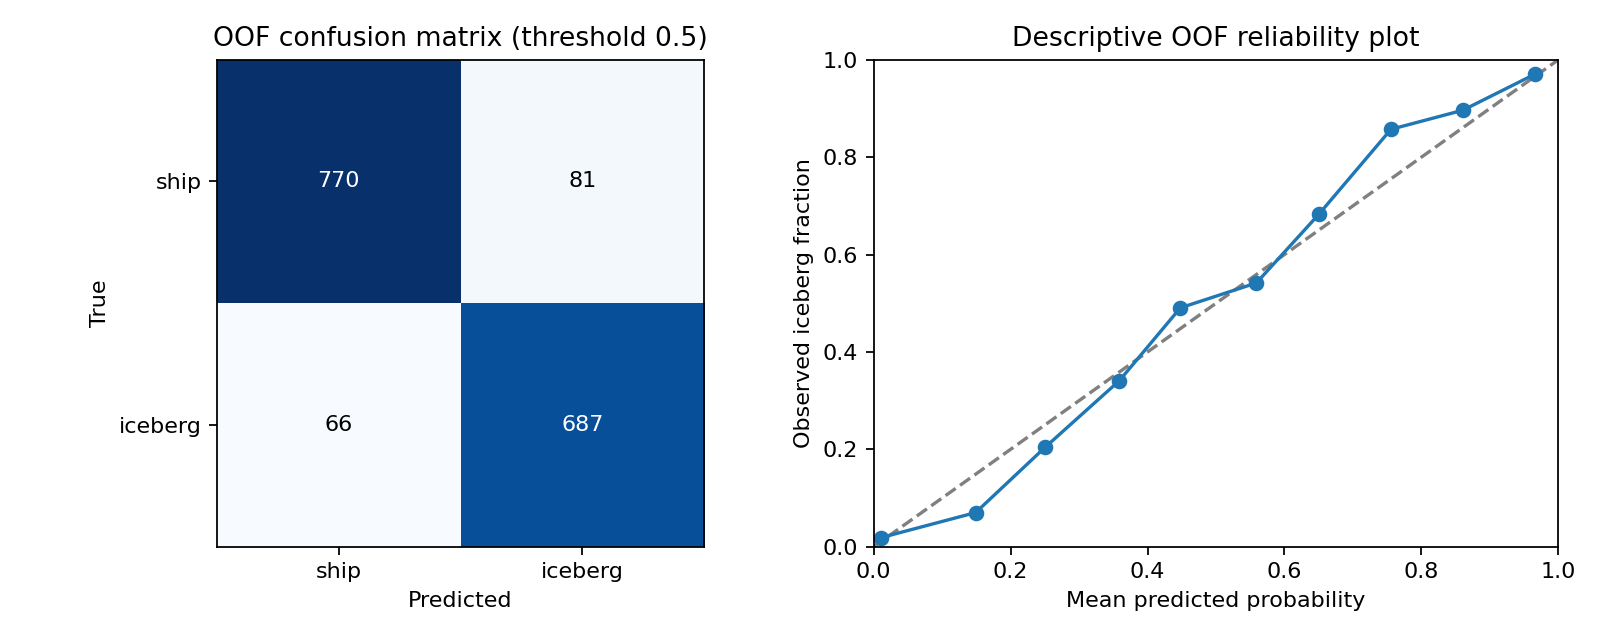
\includegraphics[width=.95\textwidth]{final/confusion_calibration.png}
\caption{V4 OOF confusion matrix and descriptive reliability plot. Calibration bins are descriptive and were not used to fit a calibration transform.}
\label{fig:confusion}
\end{figure*}

The highest-loss case is iceberg ID \texttt{37f93675}, assigned probability 0.00328, with sample loss 5.71915. Another iceberg, \texttt{3b431e27}, receives probability 0.00487 and loss 5.32475. Ship \texttt{2f881d78} receives iceberg probability 0.99137 and loss 4.75290. Figure~\ref{fig:errors} displays six high-loss cases using both channels. These examples identify failure modes for further investigation; visual appearance alone does not justify relabeling them or attributing each failure to a particular physical cause.

\begin{figure*}[t]
\centering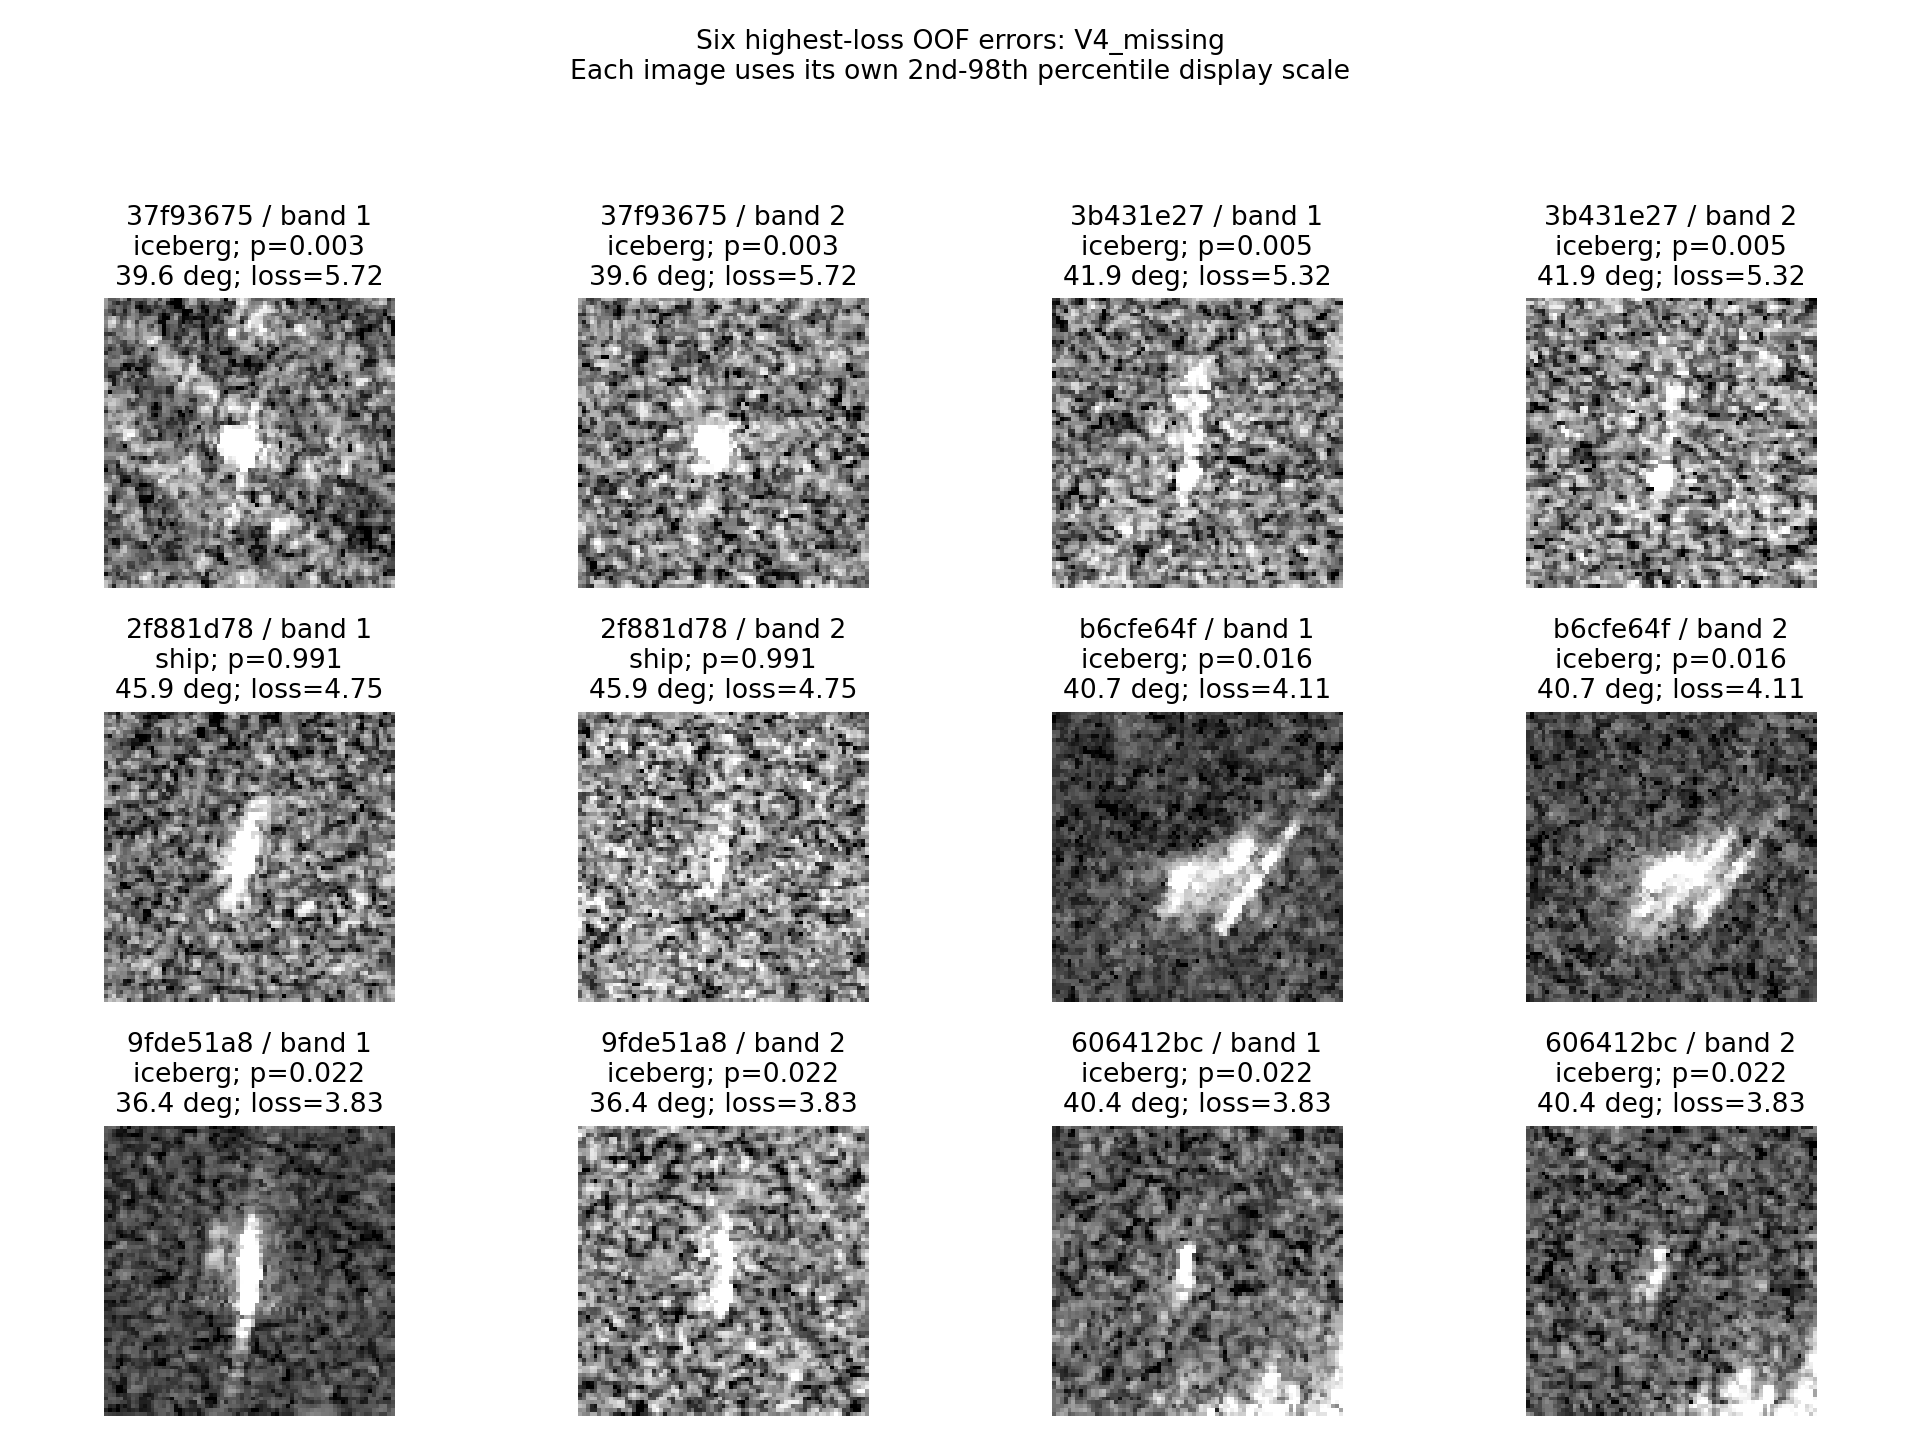
\includegraphics[width=.94\textwidth]{final/error_gallery.png}
\caption{Six V4 validation errors with the largest sample Log Loss. Probabilities refer to iceberg. Panels use independent contrast scales for visibility, so brightness should not be compared directly across panels. These are held-out predictions, not training-set predictions.}
\label{fig:errors}
\end{figure*}

\subsection{Angle-dependent performance}
Table~\ref{tab:angles} shows descriptive results in fixed angle intervals. Loss is 0.12669 for 30--35 degrees, 0.24080 for 35--40 degrees and 0.29867 for 40--50 degrees. The latter interval contains 83 errors among 640 samples. The 20--30-degree group has only one example, so its low loss is not meaningful evidence of reliable low-angle performance. All observed training angles in the final interval are below 45.94 degrees; the table does not validate extrapolation to the largest test angles.

These intervals were used for descriptive analysis after model selection, not to tune a new model or transformation. The association between angle and difficulty is not causal: image appearance, class composition and acquisition conditions may also vary across intervals. No synthetic-noise, adversarial or out-of-domain stress test has been performed. Robustness conclusions are limited to these subgroups and the existing angle-group sensitivity experiment.

\begin{table}[t]
\caption{V4 primary OOF performance by observed angle}
\label{tab:angles}\centering
\begin{tabular}{lrrr}\toprule
Angle interval (degrees) & Samples & Errors & Log Loss\\\midrule
$[20,30)$ & 1 & 0 & 0.06484\\
$[30,35)$ & 258 & 11 & 0.12669\\
$[35,40)$ & 572 & 53 & 0.24080\\
$[40,50)$ & 640 & 83 & 0.29867\\\bottomrule
\end{tabular}
\end{table}

\begin{figure*}[t]
\centering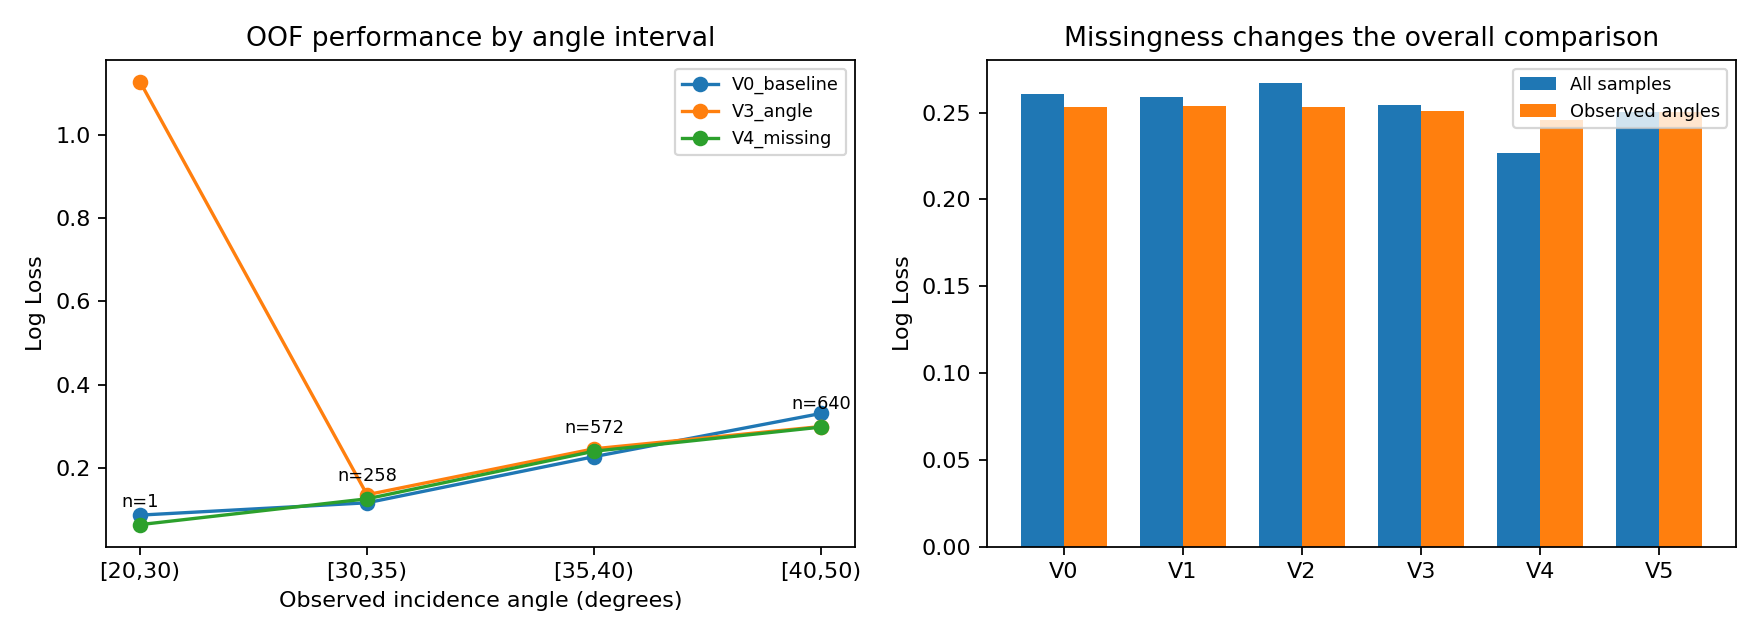
\includegraphics[width=.95\textwidth]{final/angle_robustness.png}
\caption{Left: observed-angle subgroup losses with sample counts. Right: overall and observed-angle losses across the six controlled configurations. Missingness explains a substantial part of the overall V4 improvement.}
\label{fig:angles}
\end{figure*}

\subsection{Test inference and Top-5 status}
Each retained V4 fold checkpoint uses its own saved preprocessing values to process the test images. The five iceberg probabilities are averaged with equal weights. The test JSON is streamed in batches, avoiding a full in-memory expansion of its approximately 1.52 GB text representation. All 8,424 rows are predicted, and the output is aligned to the sample submission by ID.

The generated file has columns \texttt{id,is\_iceberg}, unique and complete IDs, finite probabilities within $[0,1]$, and no missing rows. It has been re-read to verify numerical round-trip consistency. Its filename is \texttt{outputs/final/submission.csv}. The exact file and checkpoint hashes are recorded in the submission manifest.

\textbf{Kaggle late-submission Log Loss: public 0.21791; private 0.20895.} The group supplied the score receipt on November 16, 2026. It shows \texttt{submission.csv}, status ``Complete (after deadline)'', and a description identifying V4\_missing with the mean probabilities of five folds (Fig.~\ref{fig:kaggle}). The displayed precision is five decimal places. The receipt is archived with a machine-readable transcription under \texttt{results/final/}. The local file hash identifies the prepared submission; the receipt matches its filename and model description, but does not expose a remote file hash or submission ID.

These are platform-computed test scores, not the OOF score of 0.22683. Differences between OOF and Kaggle scores cannot isolate an ensembling benefit because the evaluation samples also differ. No training, calibration or selection changes were made in response to this receipt.

\textbf{Historical Top-5 score level: not reached. Formal leaderboard rank: not claimed.} The group also supplied public and private leaderboard screenshots. The displayed fifth-place public score is 0.08805 (beluga); the fifth-place private score is 0.08883 (Kohei and Medrr). Our corresponding scores are higher by 0.12986 and 0.12012, respectively (Table~\ref{tab:kagglecomparison}). Lower Log Loss is better. Thus neither board supports a historical Top-5-level performance claim. The screenshot headers identify approximately 8\% public and 92\% private evaluation portions; comparisons are made within the same board.

Kaggle staff explain that late submissions receive scores without updating the closed leaderboard \cite{kagglelate}. The receipt contains no rank, and an exact hypothetical rank cannot be inferred from the top-five screenshots. This submission establishes online-scoring availability, corresponding to the course's Case A. The instructor's treatment of late submissions remains a course-grading question; it does not change the measured gap to the historical fifth-place scores.

\begin{table}[t]
\caption{Kaggle late-submission scores versus historical fifth place}
\label{tab:kagglecomparison}\centering
\begin{tabular}{lrrr}\toprule
Board & Our Log Loss & Fifth place & Excess loss\\\midrule
Public & 0.21791 & 0.08805 & 0.12986\\
Private & 0.20895 & 0.08883 & 0.12012\\\bottomrule
\end{tabular}
\end{table}

\begin{figure*}[t]
\centering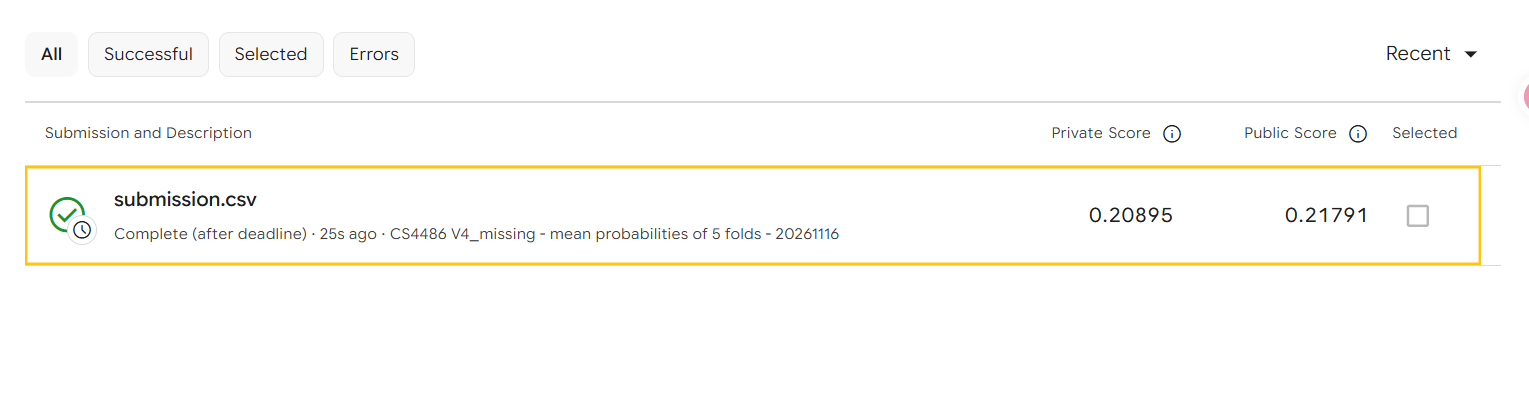
\includegraphics[width=.98\textwidth]{final/kaggle_submission_20261116.png}
\caption{Group-supplied Kaggle receipt, November 16, 2026. The left score is private (0.20895); the right score is public (0.21791). The completed entry is a late submission, not evidence of an official leaderboard rank.}
\label{fig:kaggle}
\end{figure*}

\section{AI Tool Usage Statement}
The project records substantial ChatGPT/Codex assistance. The existing log reports assistance with repository organization, EDA code and execution, validation implementation, CNN design and training code, checkpoint handling, V-series experiments, baseline replay, integrity checks and English documentation. The present work adds bundle verification, checkpoint replay in a local runtime, OOF error analysis, model selection logic, test inference, figures and drafting of this report.

These activities extend beyond language polishing. The group has supplied member responsibilities and total productive hours, recorded in Sections X and XI. These allocations identify responsibility for the work; they do not by themselves distinguish independently implemented elements from AI-assisted elements. The final statement must accurately describe what each member designed, implemented, reviewed and understood, together with the assistance received.

\pending{Each member must confirm their actual independent design/implementation work, review the technical claims, and revise this statement to match their own contribution and the course requirements.} Personal understanding is not proven by an automated test or by successful execution. Students should be able to explain fold-local preprocessing, OOF construction, the missing-angle caveat, the model architecture and the differences between local validation and leaderboard evaluation.

\section{Discussion \& Reflection}
\subsection{Effective and ineffective changes}
The experiments support a task-specific interpretation of metadata. The angle branch gives a modest primary improvement, but its advantage over V1 does not persist on the angle-group split. The missingness indicator produces the strongest pooled improvement and also modestly improves observed-angle loss. Both aspects should be reported together. A large overall gain by itself would conceal the distribution mismatch caused by complete test angles.

Higher dropout does not improve pooled loss, and flip augmentation is not consistently beneficial across the image-only and angle-fusion configurations. These negative findings illustrate why each change needs a controlled comparison. The 30-epoch limit and one seed per fold bound the conclusions: a different budget or seed distribution could alter the ranking.

The selected V4 reduces classification errors overall, but 51 samples that V0 classified correctly become errors. Twenty-five confident mistakes remain. This makes probability quality and failure-case inspection useful even after accuracy increases. The reliability plot provides a descriptive check, but it is not a guarantee of calibrated probabilities on the test distribution.

\subsection{Limitations and future work}
The principal limitations are the small labeled dataset, missingness correlated with class, incomplete acquisition metadata, a wider test-angle range, model-selection reuse of validation labels, and numerical differences between historical and current environments. The supplementary group split addresses only exact-angle association and does not establish full scene independence.

The measured Kaggle scores remain substantially above the historical Top-5 thresholds. This batch explored six configurations around a compact three-block image backbone, with one seed per fold and a 30-epoch cap. All five primary V4 runs reached that cap; their selected epochs were 25, 28, 29, 24 and 29. A larger training budget and broader model comparisons are reasonable follow-up hypotheses, but neither is proven to close the gap. The existing results cannot attribute the gap causally to a particular pipeline step or team member. Checkpoint replay and submission-format checks support implementation consistency, not optimal predictive performance.

Useful follow-up experiments would reserve an independent labeled evaluation design where feasible, evaluate multiple seeds, and test whether image features improve performance on high-angle and high-loss examples. A missingness-free training sensitivity study could help distinguish the role of the indicator from broader changes in the learned image representation. Such studies are proposals, not completed results in this report. Additional tuning should keep a clear boundary between exploratory validation and final evaluation.

\section{Reproducibility}
\subsection{Artifacts and versions}
The source snapshot used for this continuation is main commit \texttt{f8c9ff0}; the experiment bundle identifies training-code commit \texttt{c8ccc8c} \cite{repo}. The original primary folds and training implementations are preserved. The bundle contains 30 primary fold checkpoints and 15 angle-group checkpoints, all with their best-epoch parameters, preprocessing, configurations and ID lists. It omits optimizer resume states; the supplied weights support inference replay rather than continuation of the original optimization states.

The complete bundle file manifest validates 308 entries. All 45 checkpoint hashes match their supplied records. All nine experiment OOF files cover 1,604 unique training IDs with matching labels and fold assignments, and recomputed losses agree with published summaries. The raw training-file hash also matches the frozen experiment input.

The original V-series training environment uses Python 3.12.14, PyTorch 2.5.1+cpu, NumPy 2.3.5 and pandas 2.2.3 on Linux. The local continuation uses Python 3.11, PyTorch 2.9.1+cpu, NumPy 2.2.1, pandas 2.2.3 and Matplotlib 3.10.0 on Windows; the exact Python patch version and OS string are stored in \texttt{handoff\_verification.json}. CPU inference uses four threads. Although the local machine has an NVIDIA GPU, this replay does not use CUDA.

All 45 checkpoints were replayed on their held-out samples. The largest absolute probability difference from supplied OOF predictions is approximately $6.26\times10^{-7}$, below the declared $2\times10^{-6}$ replay tolerance. Each pooled replay loss also passes an absolute $2\times10^{-6}$ tolerance. These results establish numerical agreement for inference in the current environment, not bitwise equality or equivalent retraining outcomes.

\subsection{Run procedure and audit trail}
From the repository root, place the original data in \texttt{data/raw/}, restore the experiment bundle to its documented paths, and install the dependencies recorded for the continuation. Run:
\begin{verbatim}
python -m src.finalize --predict
\end{verbatim}
This audits inputs and all retained models, writes subgroup tables and error figures, selects the configuration, and creates test predictions. It performs no training and no Kaggle upload. Small aggregate evidence is written to \texttt{results/final/}; per-sample error details and submission files are written to \texttt{outputs/final/}. The provided project notes explain the files and unresolved report fields.

The training pipeline remains reproducible through the earlier V-series instructions and environment pins. Raw competition data and model files remain local or in the shared bundle, as documented in the repository. Access to the private source repository must be arranged for the course evaluator. Machine-readable hashes identify the exact inputs and outputs used for the reported analysis.

\section{Student Bio and Self-Reflection}
Member names, Student IDs, responsibilities and total productive hours below were supplied by the group. Step numbers refer to the team's twelve-step project plan. Biographies and personal reflections remain to be supplied by each member.
\subsection{Group Leader: Huang Yifan}
\textbf{Student ID:} 72400438. \textbf{Actual productive hours:} 8.
\textbf{Biography:} \pending{Background and interests.}
\textbf{Self-reflection:} \pending{What the member learned and what they would change.}
\textbf{Contribution justification:} Responsible for Steps 4--6: exploratory data analysis of classes, radar images, missing angles and duplicate or similar samples; the fixed five-fold validation design and fold assignments, with preprocessing fitted on training folds; and the two-channel CNN baseline, including training, early stopping, saved models and OOF evaluation. These tasks established the dataset evidence, shared validation protocol and baseline used by the subsequent experiments. Supporting outputs include the EDA summaries and figures, fixed split files, baseline scores, learning curves and OOF predictions. The reported 8 hours cover these steps jointly.
\subsection{Group Member A: Zheng Hongyu}
\textbf{Student ID:} 72400229. \textbf{Actual productive hours:} 6.
\textbf{Biography:} \pending{Background and interests.}
\textbf{Self-reflection:} \pending{Personal reflection.}
\textbf{Contribution justification:} Responsible for Steps 9--11: error and robustness analysis of confident mistakes, missing angles and angle-dependent performance; final-model selection from validation evidence, generation of test probabilities and the subsequent Kaggle upload; and preparation of the course-format report, including results, citations, AI-use disclosure and contribution records. Supporting outputs include the error-case figures, subgroup metrics, model-selection record, submission CSV, completed Kaggle score receipt and this report draft. The reported 6 hours cover these steps jointly and have not been automatically increased for later activity. The course Top-5 interpretation and remaining personal/report fields are still pending.
\subsection{Group Member B: Hachiware}
\textbf{Student ID:} 72400463. \textbf{Actual productive hours:} 7.
\textbf{Biography:} \pending{Background and interests.}
\textbf{Self-reflection:} \pending{Personal reflection.}
\textbf{Contribution justification:} Responsible for Steps 7--8: controlled model-improvement experiments involving augmentation, regularization and angle fusion, followed by comparisons and ablations on the same fixed folds, including the missing-angle feature. The resulting experiment configurations, training results and comparison tables provide the evidence for the final model choice. Supporting outputs are the V0--V5 results, OOF predictions, saved fold checkpoints and supplementary grouped comparisons in the experiment bundle. The reported 7 hours cover these steps jointly.

\section{Relative Contribution}
The group reports 8 actual productive hours for Huang Yifan (Steps 4--6), 6 for Zheng Hongyu (Steps 9--11), and 7 for Hachiware (Steps 7--8), totaling 21 hours. These are reported human work totals, not automated training or inference runtime. The allocation of each total across the five course-template categories has not yet been supplied. Table~\ref{tab:contribution} records the known totals and leaves the category-level hours pending; ``Pending'' does not mean zero. Step 12 (presentation and reproduction check) is not claimed as completed by this allocation.
\begin{table*}[t]
\caption{Reported actual productive hours; category-level allocation pending}
\label{tab:contribution}\centering\renewcommand{\arraystretch}{1.3}
\begin{tabularx}{.98\textwidth}{lXXXXXc}\toprule
Member & Data analysis \& validation & Baseline & Model improvement & Final experiments \& tuning & Report \& presentation & Total\\\midrule
Huang Yifan & Pending & Pending & Pending & Pending & Pending & 8\\
Zheng Hongyu & Pending & Pending & Pending & Pending & Pending & 6\\
Hachiware & Pending & Pending & Pending & Pending & Pending & 7\\\midrule
Team total & Pending & Pending & Pending & Pending & Pending & 21\\\bottomrule
\end{tabularx}
\end{table*}

\section*{Team Leader Attestation}
\pending{To be completed only after contribution entries have been confirmed.}
``I, Huang Yifan, confirm that the contributions listed above accurately reflect the work completed by each team member.''\\
Signed: \rule{5cm}{0.4pt}

\begin{thebibliography}{9}
\bibitem{kaggle} Kaggle, ``Statoil/C-CORE Iceberg Classifier Challenge,'' competition overview and evaluation. [Online]. Available: \url{https://www.kaggle.com/competitions/statoil-iceberg-classifier-challenge}.
\bibitem{data} Kaggle, ``Statoil/C-CORE Iceberg Classifier Challenge: Data.'' [Online]. Available: \url{https://www.kaggle.com/competitions/statoil-iceberg-classifier-challenge/data}.
\bibitem{bce} PyTorch, ``BCEWithLogitsLoss,'' documentation. [Online]. Available: \url{https://docs.pytorch.org/docs/stable/generated/torch.nn.BCEWithLogitsLoss.html}.
\bibitem{randomness} PyTorch, ``Reproducibility,'' documentation. [Online]. Available: \url{https://docs.pytorch.org/docs/stable/notes/randomness.html}.
\bibitem{repo} CS4486 project repository, source snapshot \texttt{f8c9ff0}, V-series code \texttt{c8ccc8c}, and accompanying experiment bundle, Nov. 15, 2026. [Online]. Available: \url{https://github.com/YifanHuang-if/cs4486-iceberg}.
\bibitem{kagglelate} A. Howard (Kaggle staff), response to ``Enabling late submissions for community competition,'' Kaggle. [Online]. Available: \url{https://www.kaggle.com/competition-hosting/403715}. Accessed Nov. 16, 2026.
\end{thebibliography}
\end{document}
